\documentclass[10pt,a4paper]{beamer}
\usepackage[utf8]{inputenc}
\usepackage[T1]{fontenc}
\usepackage[francais]{babel}
\usepackage{amsmath}
\usepackage{amsfonts}
\usepackage{hyperref}

\usepackage{tikz}

\usepackage{pdflscape}
\usepackage{pdfpages}
\usetheme{Warsaw}

\subtitle{Développement Web sur le framework Ruby on Rails}
\title{Soutenance Finale}
\author{Jaussoin Timothée \\ \and Maître de Stage Floris Vlasveld \\ \and Enseignant Responsable Normand Nicolas}
\institute{Polytech Nantes - Département Informatique}

\begin{document}
\begin{frame}
  \titlepage
\end{frame}

\section{About the Internship}

\begin{frame}{About the internship}
  \begin{itemize}
    \item 6 months
    \item Inspire, Utrecht, The Netherlands
  \end{itemize}
  
  \begin{block}{Topic}
    \begin{itemize}
      \item Web Development on Ruby on Rails
      \item Frontend oriented (Javascript, HTML5, CSS)
    \end{itemize}
  \end{block}

  \begin{block}{Project}
    \begin{itemize}
      \item Calibris - Questionnaire Manager
      \item Add new features, refactor and optimize the source-code
    \end{itemize}
  \end{block}
\end{frame}

\subsection{Inspire}

\begin{frame}{Inspire}

  \begin{figure}[htp]
  \centering
  
\includegraphics[width=0.3\textwidth]{../img/logo.png}
  \end{figure}

  \begin{itemize}
    \item Located in Utrecht, The Netherlands
    \item Created in 2011
    \item Projects developped on the Ruby on Rails framework
    \item Working with parts of the Agile methods
  \end{itemize}
  
  \begin{block}{Team}
    \begin{itemize}
      \item 4 developpers
      \item 2 managers
      \item … and some freelancers
    \end{itemize}
  \end{block}
\end{frame}

\subsection{Inspire -- My Role}

\begin{frame}{Inspire -- My Role}

  \begin{itemize}
    \item Working as a Ruby on Rails -- Frontend developer
    \item Already worked on the framework (last internship)
  \end{itemize}
  
  \begin{block}{Organisationnal part}
    \begin{itemize}
      \item Organize meetings with members of the team (for Calibris)
      \item Giving some feedbacks (stand-up, team meeting)
    \end{itemize}
  \end{block}
  
  \begin{block}{Technical part}
    \begin{itemize}
      \item Helping on frontend optimisations (Javascript, HTML5)… and backend (database side)
      \item Giving a fresh view on some issues (with my experience)
    \end{itemize}
  \end{block}
  
  \begin{block}{Human part}
    \begin{itemize}
      \item Helping with the daily team issues
      \item … using the Agile methods
    \end{itemize}
  \end{block}
\end{frame}

\section{To begin with…}

\subsection{Ruby on Rails}

\begin{frame}{To begin with… Ruby on Rails}
  \begin{figure}[htp]
  \centering
  
\includegraphics[width=0.2\textwidth]{../img/logo_rails.png}
  \end{figure}

  \begin{itemize}
    \item Web oriented framework, first version in 2004
    \item Based on the Ruby language
  \end{itemize}

  \begin{block}{Technical overview}
    \begin{itemize}
      \item MVC oriented
      \item REST
      \item Object-relationnal Mapping -- Active record
      \item Package--Dependency system
    \end{itemize}
  \end{block}
\end{frame}

\subsection{The tests}

\begin{frame}{To begin with… the tests}

  \begin{block}{RSpec}
  	Unit test system
    \begin{itemize}
      \item Can test the models, controllers and views
      \item Two levels : 
		\begin{itemize}
		  \item Defining the context
		  \item The proof itself
		\end{itemize}
    \end{itemize}
  \end{block}
  
  \begin{block}{Cucumber}
  	Unit test system
    \begin{itemize}
      \item Define the "user behaviour"
      \item Frontend navigation (forms, links…)
    \end{itemize}
  \end{block}
\end{frame}

\subsection{Agile}

\begin{frame}{To begin with… Agile}

	\begin{figure}[htp]
	\centering
	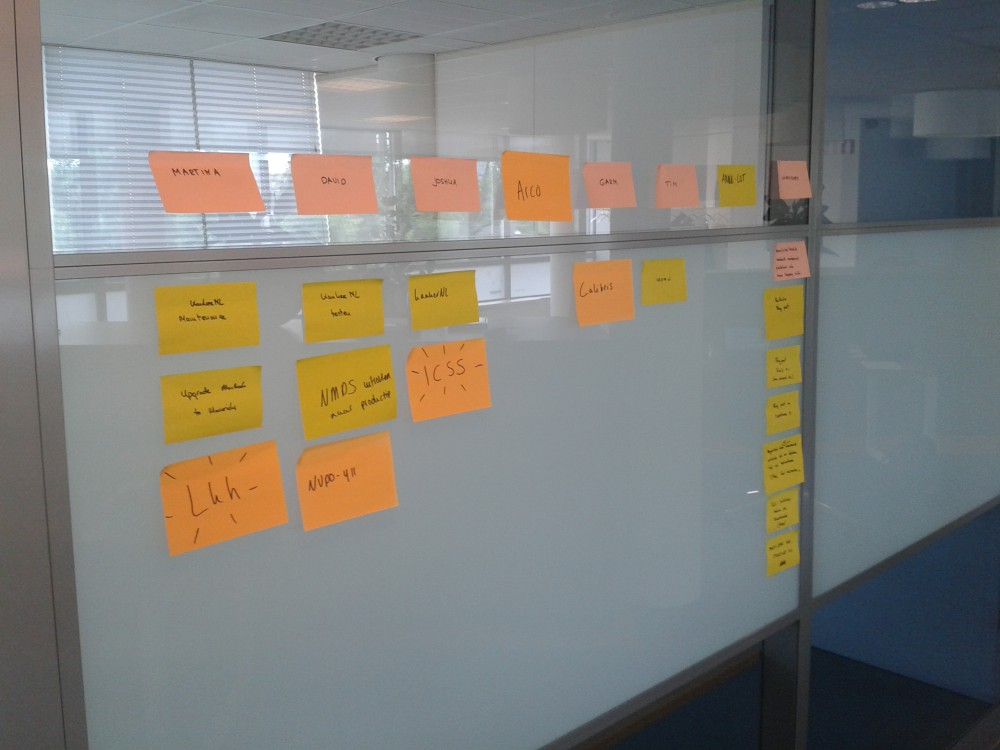
\includegraphics[scale=.15]{../img/agile1.jpg}
	 \label{fig.agile1}
	\end{figure}

  \begin{itemize}
    \item General overview using the ``Scrum board''
    \item Detailled overview on Jira
  \end{itemize}
  
\end{frame}

\subsection{Jira, Github}

\begin{frame}{To begin with… Jira, GitHub}

  \begin{block}{Jira}
  	Project manager
    \begin{itemize}
      \item Manage the issues, per project
      \item Check the progression, velocity
      \item Track the time (Tempo module)
    \end{itemize}
  \end{block}

  \begin{block}{Github}
  	Manage the sourcecode
    \begin{itemize}
      \item Online repository management system
      \item Private repository
      \item Pull request
      \item Linked with Jira
    \end{itemize}
  \end{block}
\end{frame}

\section{Planning}

\begin{frame}{Planning -- Gantt Initial}

\begin{landscape}
\begin{figure}[htp] \centering{
	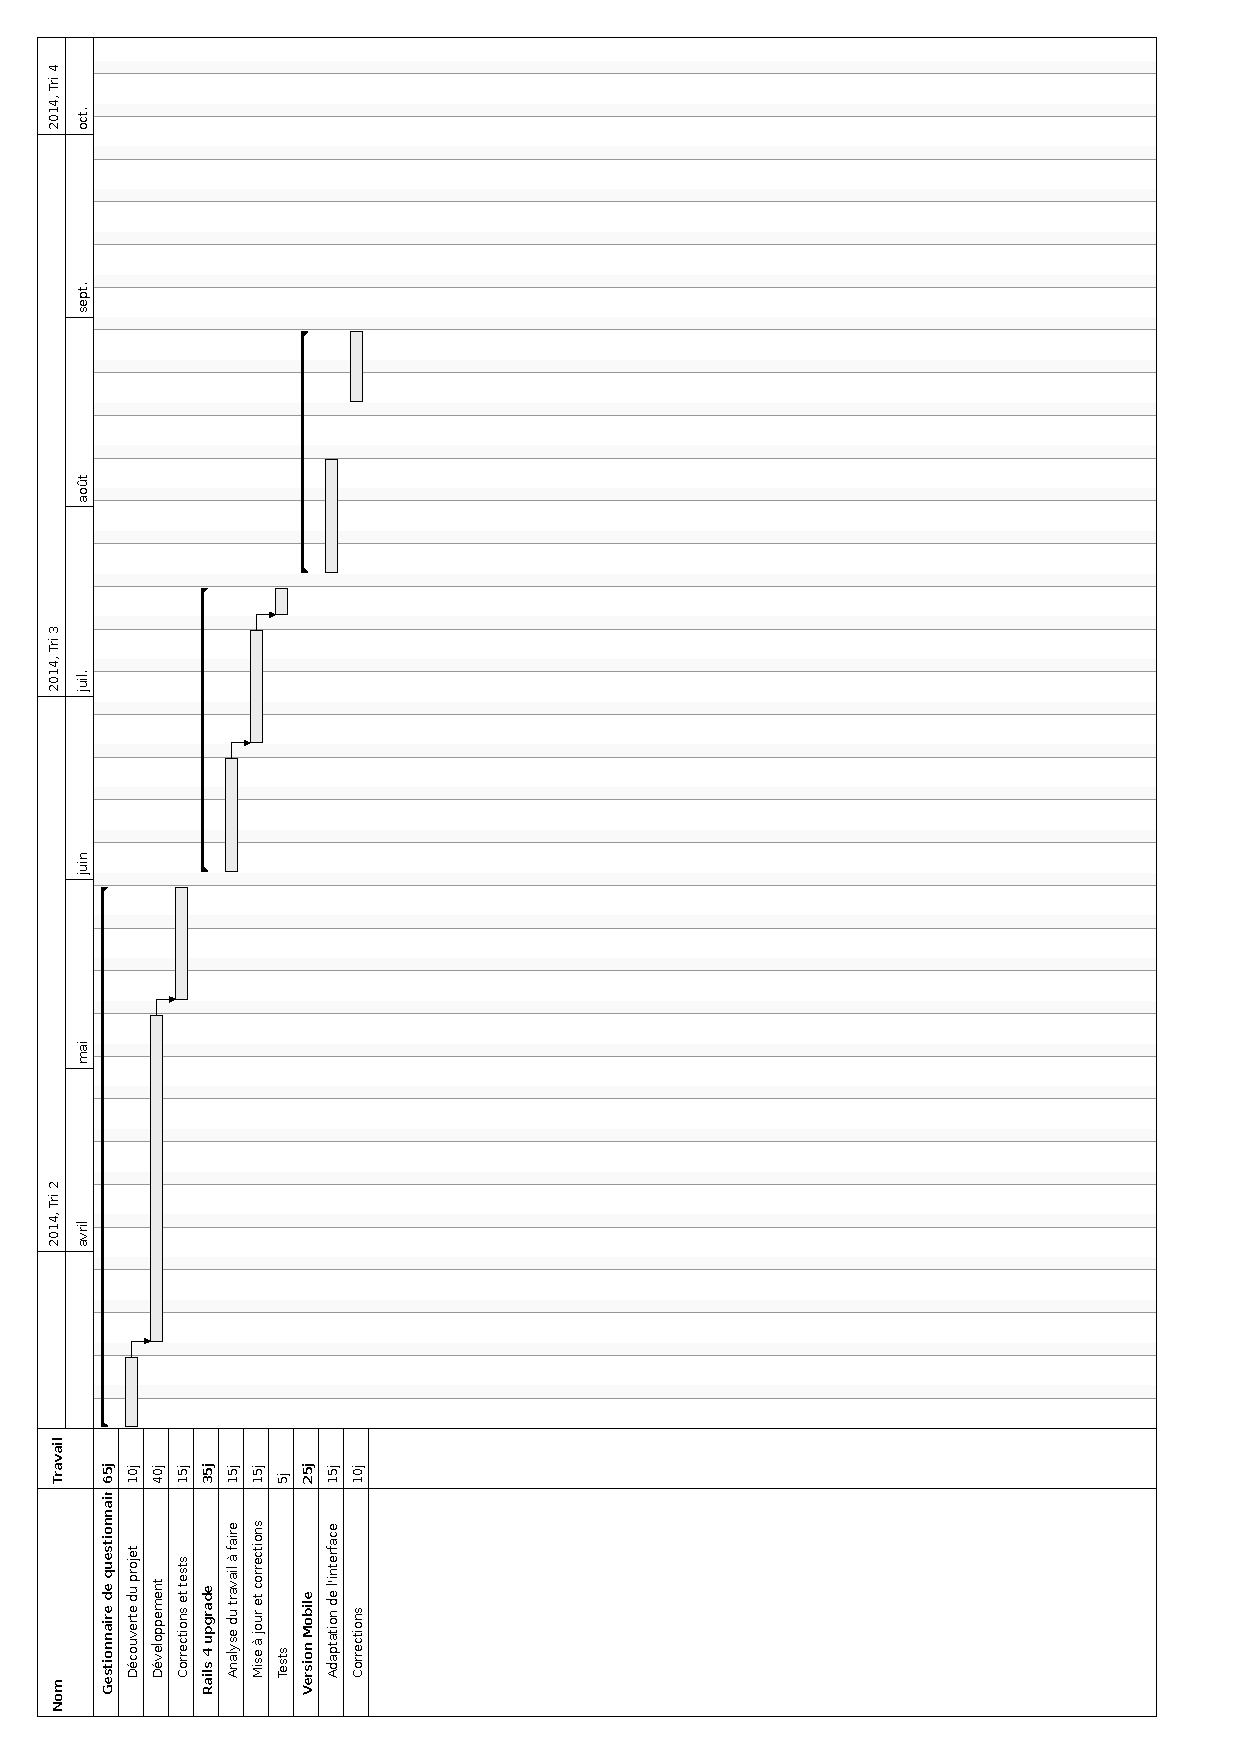
\includegraphics[scale=0.38, angle=270]{../gantt_initial.pdf}}
\end{figure}
\end{landscape}

\end{frame}

\begin{frame}{Planning -- Gantt Final}

\begin{landscape}
\begin{figure}[htp] \centering{
	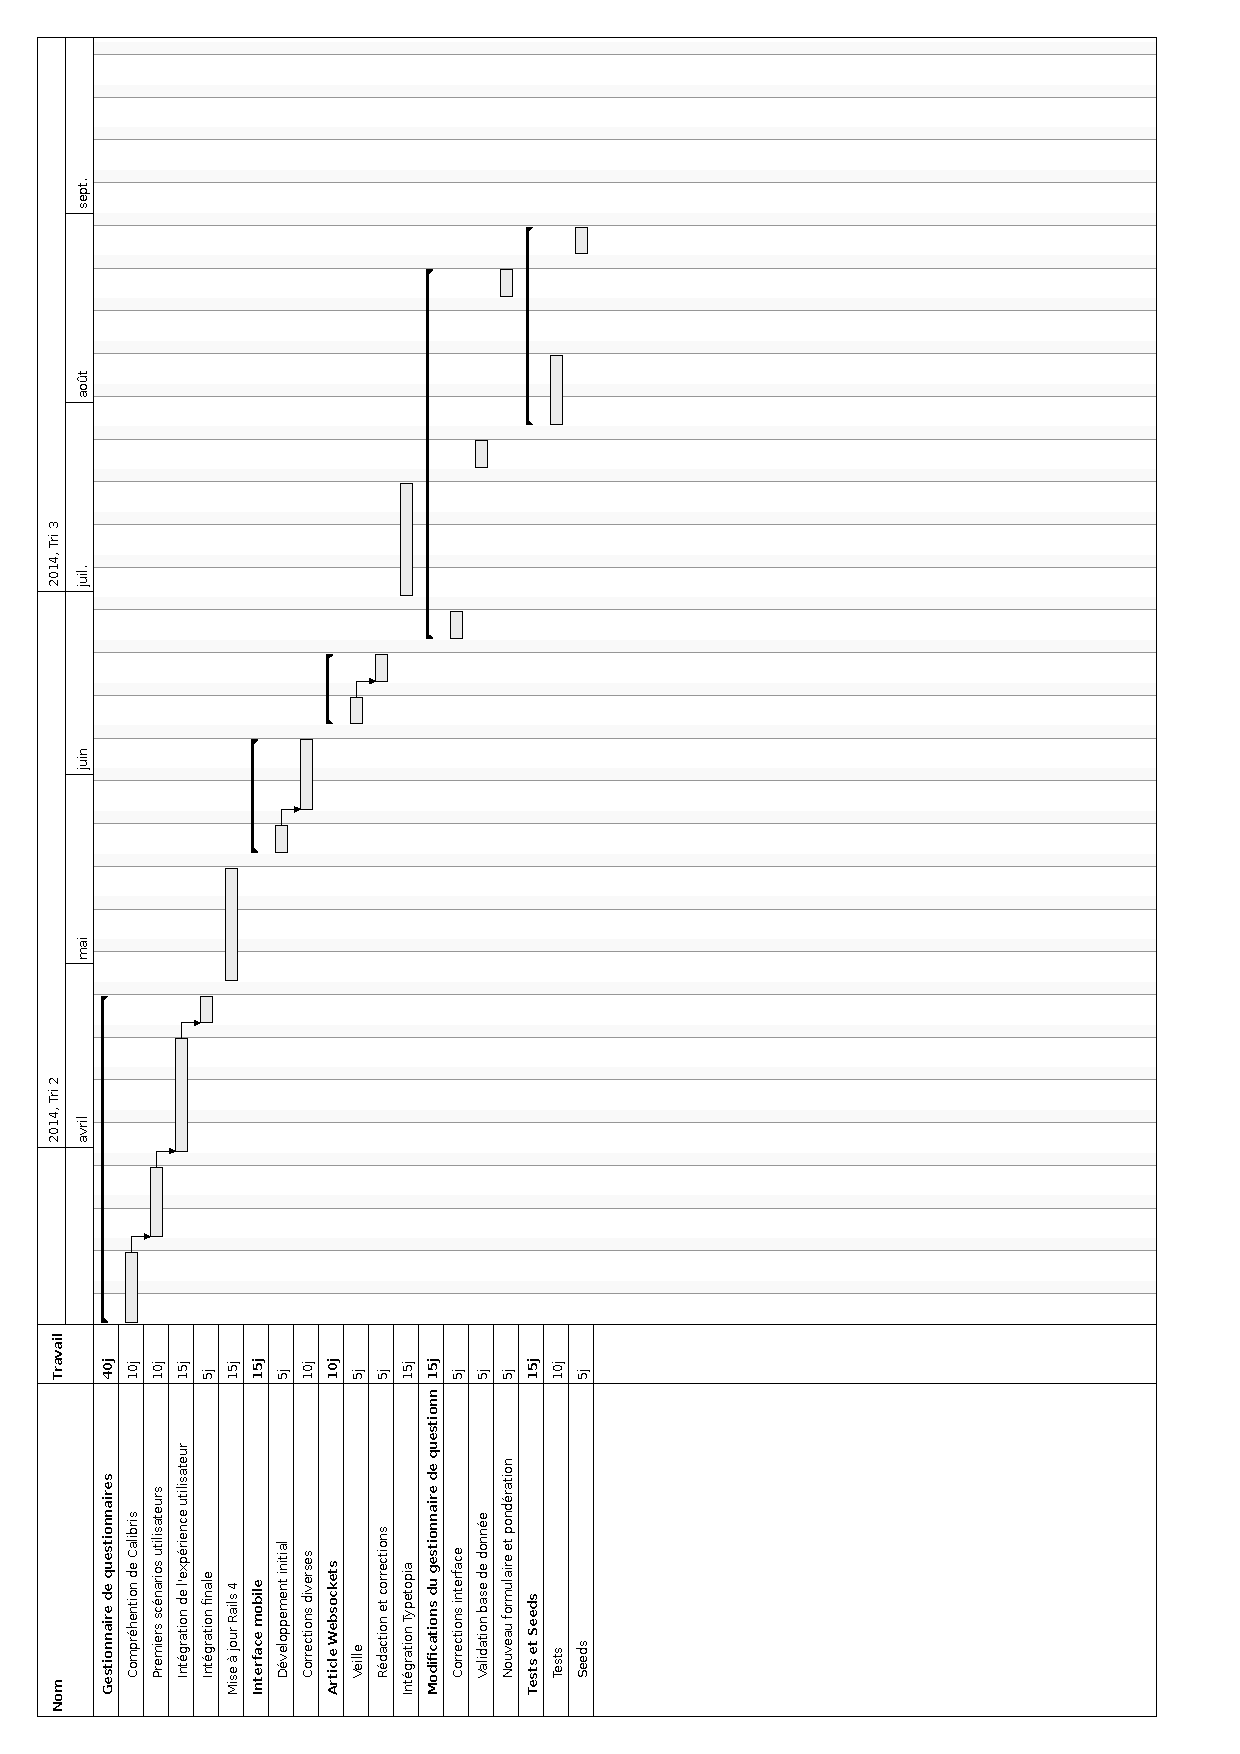
\includegraphics[scale=0.38, angle=270]{../gantt_final.pdf}}
\end{figure}
\end{landscape}

\end{frame}

\section{Calibris}
\subsection{Overview}

\begin{frame}{Calibris - Overview}

  \begin{figure}[htp]
  \centering
  
\includegraphics[scale=.50]{../img/calibris.jpg}
  \end{figure}
  
  \begin{itemize}
    \item Questionnaire manager
    \item Now used by several clients
  \end{itemize}

	\begin{figure}[h]
	   \centering
	\begin{tikzpicture}
	\begin{scope}[xscale=1,yscale=1]
	% description et nommage des noeuds 
	\node (A) at (0,0) [circle, draw] {\Large{Calibris}};
	\node (I) at (0,2) [rectangle,draw] {Inspire};
	\node (C1) at (-3,1) [rectangle,draw] {Calibris};
	\node (C2) at (-3,0) [rectangle,draw] {Innergo};
	\node (C3) at (-3,-1) [rectangle,draw] {ICSS};
	\node (T) at (-3,2) {\textbf{Clients/Administrateurs}};
	\node (T) at (3,2) {\textbf{Utilisateurs passifs}};
	\node (R) at (3,0) [rectangle,draw] {Respondents};
	\draw[dashed, ->]  (I) -- (A);
	\draw (C1) -- (A);
	\draw (C2) -- (A);
	\draw (C3) -- (A);
	\draw[->] (R) -- (A);
	\end{scope}
	\end{tikzpicture}
	\caption{General overview of the Calibris users} 
	\label{fig.calibris_clients}
	\end{figure}
\end{frame}

\begin{frame}{Calibris - Overview}
  \begin{figure}[htp]
  \centering
  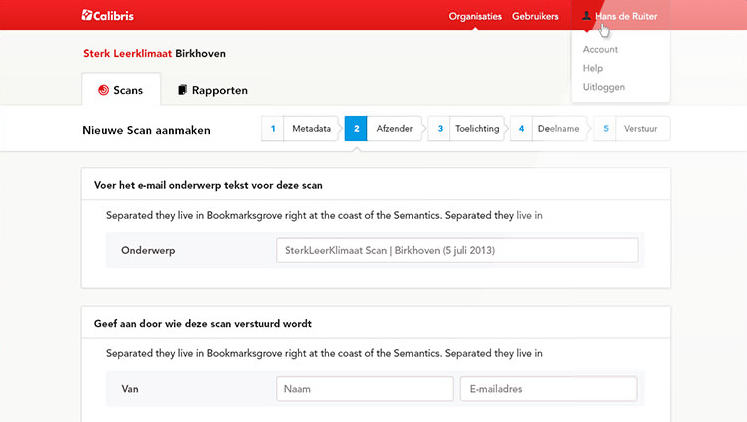
\includegraphics[scale=0.4]{../img/calibris1.png}
   \caption{Creating a new survey on Calibris}
   \label{fig.calibris1}
  \end{figure}
\end{frame}
  
\begin{frame}{Calibris - Overview}
  \begin{figure}[htp]
  \centering
  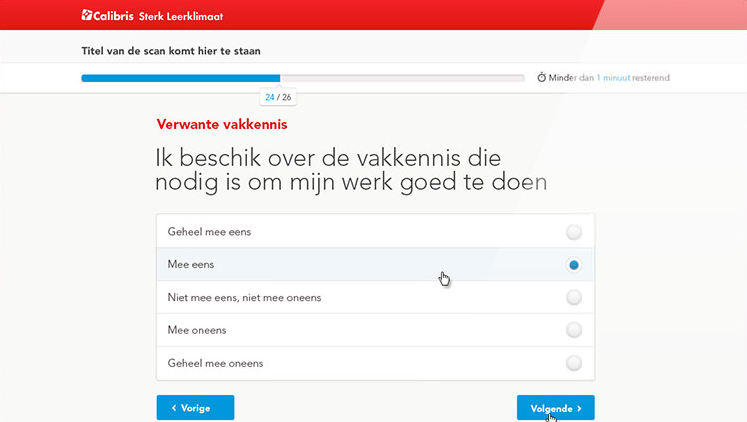
\includegraphics[scale=0.4]{../img/calibris2.png}
   \caption{Aswering a questionnaire on Calibris}
   \label{fig.calibris2}
  \end{figure}
\end{frame}

\subsection{Projects}

\begin{frame}{Projects}
  \begin{description}
    \item[Project 1] Questionnaire Manager
    \item[Project 2] Update to Rails 4.1
    \item[Project 3] Mobile version
    \item[Project 4] Improvements on the questionnaire editor
    \item[Project 5] Tests and ``seeds''
  \end{description}
  But also… fixing issues and participating with the team in the daily updates and improvements of Calibris.
\end{frame}

\subsubsection{Questionnaire Manager}

\begin{frame}{Questionnaire Manager}
  \begin{block}{Questionnaires structure}
    \begin{itemize}
      \item Categories
      \item Clusters
      \item Questions 
    \end{itemize}
  \end{block}

  \begin{block}{To Do}
    \begin{itemize}
      \item Implement basic CRUD (Create, Read, Update and Delete) actions 
      \item Add inline editing
      \item Add drag\&drop reordering 
      \item Link it with the all application
    \end{itemize}
  \end{block}
  
  \begin{block}{}
    \begin{itemize}
      \item 8 weeks
      \item Merged in the trunk
    \end{itemize}
  \end{block}
\end{frame}

\begin{frame}{Questionnaire Manager - Implementation}
  \begin{itemize}
    \item Using \texttt{awesome\_nested\_set} to handle the questionnaires structures
    \item Using the Rails \texttt{remotes} to send and receive dynamicaly parts of the page
    \item Using jQuery sortable to reorder dynamicaly the categories, clusters and questions
  \end{itemize}
  
  \begin{figure}[htp]
  \centering
  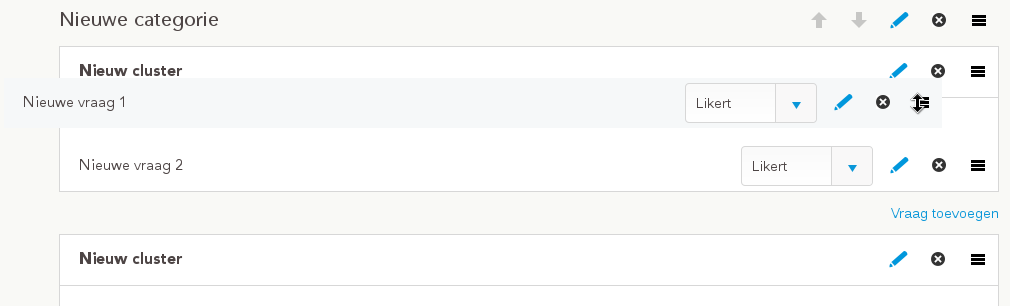
\includegraphics[scale=0.3]{../img/calibris_drag_drop.png}
   \caption{Drag\&Drop a question}
  \end{figure}
\end{frame}

\subsubsection{Rails 4.1 Upgrade}

\begin{frame}{Rails 4.1 Upgrade}
  \begin{block}{To Do}
    \begin{enumerate}
      \item Update the Gemfile
      \item Fixing the critical bugs
      \item Running the test suite
      \item Fixing the remaining bugs
    \end{enumerate}
  \end{block}
  
  \begin{block}{}
    \begin{itemize}
      \item 3 weeks
      \item Trunk updated
    \end{itemize}
  \end{block}
\end{frame}

\subsubsection{Mobile version}

\begin{frame}{Mobile version}
  \begin{block}{To Do}
    \begin{itemize}
      \item Make the CSS responsive (using CSS3 media-queries)
      \item Check on desktop 
      \item Check the size and resolution of the elements
      \item Check on iOS, Android
      \item Fix the remaining issues 
    \end{itemize}
  \end{block}
  
  \begin{block}{}
    \begin{itemize}
      \item 1 weeks + 2 more weeks for remaining issues
      \item Merged in the trunk
    \end{itemize}
  \end{block}
\end{frame}

\begin{frame}

\begin{figure}[htp]
\centering
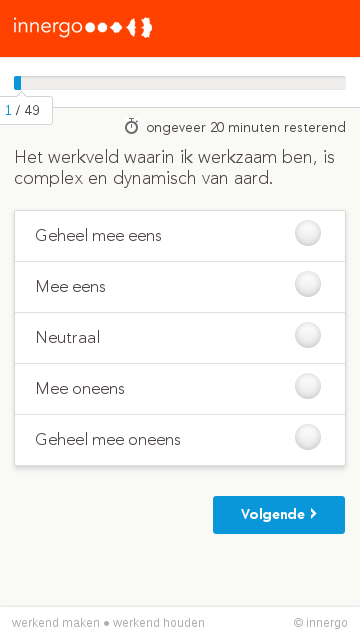
\includegraphics[scale=0.32]{../img/calibris3.png}
 \caption{The respondent view on mobile}
 \label{fig.calibris3}
\end{figure}

\end{frame}

\subsubsection{Questionnaire editor improvement}

\begin{frame}{Questionnaire editor improvement}
	\begin{figure}[htp]
	\centering
	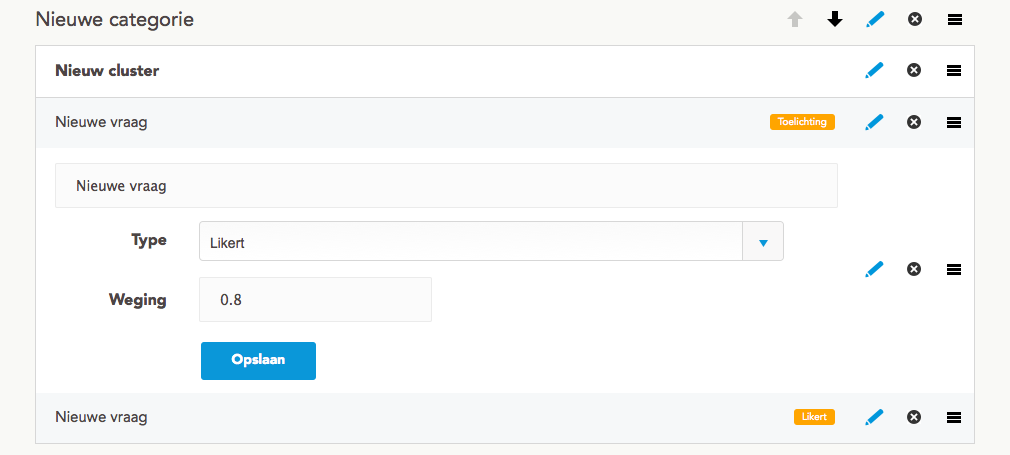
\includegraphics[scale=.32]{../img/editor.png}
	 \caption{New question edition form}
	 \label{fig.editor}
	\end{figure}
\end{frame}

\begin{frame}{Questionnaire editor improvement}
  \begin{block}{To Do}
    \begin{itemize}
      \item Refactor the question form
      \item Add a \texttt{weight} attribute
      \item Clean the CSS, Ruby code
    \end{itemize}
  \end{block}
  
  \begin{block}{}
    \begin{itemize}
      \item 3 weeks
      \item Merged in the trunk
    \end{itemize}
  \end{block}
\end{frame}

\subsubsection{Tests and seeds}

\begin{frame}{Tests and seeds}
  \begin{block}{To Do}
    \begin{itemize}
      \item Adding new RSpec and Cucumber tests to cover the code
      \item Fix and rewrite the ``seeds'' to fill properly the database
    \end{itemize}
  \end{block}
  
  \begin{block}{}
    \begin{itemize}
      \item 3 weeks
      \item Merged in the trunk
    \end{itemize}
  \end{block}
\end{frame}

\section{Summary}

\subsection{Feedback}

\begin{frame}{Feedback}
  \begin{block}{Technical part}
    \begin{itemize}
      \item Strengthening my knowledge in Rails… but also in general Web development (concepts…)
      \item I do not want to be specialized in one technologie yet
    \end{itemize}
  \end{block}
  
  \begin{block}{Internship topic}
    \begin{itemize}
      \item Interesting
      \item Worked on my weakness (frontend side)
      \item Working on a big project… but from several unique perspectives
    \end{itemize}
  \end{block}
  
  \begin{block}{Whithin the team}
    \begin{itemize}
      \item Good feeling
      \item Try to complete what was missing
    \end{itemize}
  \end{block}
\end{frame}

\subsection{General overview}

\begin{frame}{General overview}
	\begin{itemize}
	  \item The Web is still not seen as a serious topic to work on 
      \begin{itemize}
        \item No serious courses in 5 years (only the network aspect)
        \item Backend (REST, API, i18n, encoding, database query…), frontend (Javascript, Ajax, DOM, HTML, CSS), optimization (long polling, sockets, memory management)…
      \end{itemize}

	  \item Need to learn all the things by myself
      \begin{itemize}
        \item Personnal project 
        \item Internships
      \end{itemize}
      
      \item … to complete some significants gaps
      \begin{itemize}
        \item Code management, bug tracker
        \item Architectural decisions 
        \item Packaging, deployment
        \item Following the standards
      \end{itemize}
	\end{itemize}
	
	The courses give some bases, teach you how to learn… you have to do your best to fill the gaps :)
\end{frame}

\subsection{Summary}

\begin{frame}{Summary}
    \begin{block}{Skills}
    \begin{itemize}
      \item Rails environment comprehension
      \item Frontend technologies (Javascript, CSS3)
      \item Organisation (Jira, Agile)
      \item Code management (Git, GitHub)
    \end{itemize}
  \end{block}
  
  \begin{itemize}
    \item Calibris, a full stack Rails project 
    \item Daily improvements and fixes
    \item Take part of a team
    \item Blog post
  \end{itemize}
\end{frame}

\end{document}